\PassOptionsToPackage{unicode=true}{hyperref} % options for packages loaded elsewhere
\PassOptionsToPackage{hyphens}{url}
%
\documentclass[]{book}
\usepackage{lmodern}
\usepackage{amssymb,amsmath}
\usepackage{ifxetex,ifluatex}
\usepackage{fixltx2e} % provides \textsubscript
\ifnum 0\ifxetex 1\fi\ifluatex 1\fi=0 % if pdftex
  \usepackage[T1]{fontenc}
  \usepackage[utf8]{inputenc}
  \usepackage{textcomp} % provides euro and other symbols
\else % if luatex or xelatex
  \usepackage{unicode-math}
  \defaultfontfeatures{Ligatures=TeX,Scale=MatchLowercase}
\fi
% use upquote if available, for straight quotes in verbatim environments
\IfFileExists{upquote.sty}{\usepackage{upquote}}{}
% use microtype if available
\IfFileExists{microtype.sty}{%
\usepackage[]{microtype}
\UseMicrotypeSet[protrusion]{basicmath} % disable protrusion for tt fonts
}{}
\IfFileExists{parskip.sty}{%
\usepackage{parskip}
}{% else
\setlength{\parindent}{0pt}
\setlength{\parskip}{6pt plus 2pt minus 1pt}
}
\usepackage{hyperref}
\hypersetup{
            pdftitle={Network Analysis in R},
            pdfauthor={Robert Wiederstein},
            pdfborder={0 0 0},
            breaklinks=true}
\urlstyle{same}  % don't use monospace font for urls
\usepackage{color}
\usepackage{fancyvrb}
\newcommand{\VerbBar}{|}
\newcommand{\VERB}{\Verb[commandchars=\\\{\}]}
\DefineVerbatimEnvironment{Highlighting}{Verbatim}{commandchars=\\\{\}}
% Add ',fontsize=\small' for more characters per line
\usepackage{framed}
\definecolor{shadecolor}{RGB}{248,248,248}
\newenvironment{Shaded}{\begin{snugshade}}{\end{snugshade}}
\newcommand{\AlertTok}[1]{\textcolor[rgb]{0.94,0.16,0.16}{#1}}
\newcommand{\AnnotationTok}[1]{\textcolor[rgb]{0.56,0.35,0.01}{\textbf{\textit{#1}}}}
\newcommand{\AttributeTok}[1]{\textcolor[rgb]{0.77,0.63,0.00}{#1}}
\newcommand{\BaseNTok}[1]{\textcolor[rgb]{0.00,0.00,0.81}{#1}}
\newcommand{\BuiltInTok}[1]{#1}
\newcommand{\CharTok}[1]{\textcolor[rgb]{0.31,0.60,0.02}{#1}}
\newcommand{\CommentTok}[1]{\textcolor[rgb]{0.56,0.35,0.01}{\textit{#1}}}
\newcommand{\CommentVarTok}[1]{\textcolor[rgb]{0.56,0.35,0.01}{\textbf{\textit{#1}}}}
\newcommand{\ConstantTok}[1]{\textcolor[rgb]{0.00,0.00,0.00}{#1}}
\newcommand{\ControlFlowTok}[1]{\textcolor[rgb]{0.13,0.29,0.53}{\textbf{#1}}}
\newcommand{\DataTypeTok}[1]{\textcolor[rgb]{0.13,0.29,0.53}{#1}}
\newcommand{\DecValTok}[1]{\textcolor[rgb]{0.00,0.00,0.81}{#1}}
\newcommand{\DocumentationTok}[1]{\textcolor[rgb]{0.56,0.35,0.01}{\textbf{\textit{#1}}}}
\newcommand{\ErrorTok}[1]{\textcolor[rgb]{0.64,0.00,0.00}{\textbf{#1}}}
\newcommand{\ExtensionTok}[1]{#1}
\newcommand{\FloatTok}[1]{\textcolor[rgb]{0.00,0.00,0.81}{#1}}
\newcommand{\FunctionTok}[1]{\textcolor[rgb]{0.00,0.00,0.00}{#1}}
\newcommand{\ImportTok}[1]{#1}
\newcommand{\InformationTok}[1]{\textcolor[rgb]{0.56,0.35,0.01}{\textbf{\textit{#1}}}}
\newcommand{\KeywordTok}[1]{\textcolor[rgb]{0.13,0.29,0.53}{\textbf{#1}}}
\newcommand{\NormalTok}[1]{#1}
\newcommand{\OperatorTok}[1]{\textcolor[rgb]{0.81,0.36,0.00}{\textbf{#1}}}
\newcommand{\OtherTok}[1]{\textcolor[rgb]{0.56,0.35,0.01}{#1}}
\newcommand{\PreprocessorTok}[1]{\textcolor[rgb]{0.56,0.35,0.01}{\textit{#1}}}
\newcommand{\RegionMarkerTok}[1]{#1}
\newcommand{\SpecialCharTok}[1]{\textcolor[rgb]{0.00,0.00,0.00}{#1}}
\newcommand{\SpecialStringTok}[1]{\textcolor[rgb]{0.31,0.60,0.02}{#1}}
\newcommand{\StringTok}[1]{\textcolor[rgb]{0.31,0.60,0.02}{#1}}
\newcommand{\VariableTok}[1]{\textcolor[rgb]{0.00,0.00,0.00}{#1}}
\newcommand{\VerbatimStringTok}[1]{\textcolor[rgb]{0.31,0.60,0.02}{#1}}
\newcommand{\WarningTok}[1]{\textcolor[rgb]{0.56,0.35,0.01}{\textbf{\textit{#1}}}}
\usepackage{longtable,booktabs}
% Fix footnotes in tables (requires footnote package)
\IfFileExists{footnote.sty}{\usepackage{footnote}\makesavenoteenv{longtable}}{}
\usepackage{graphicx,grffile}
\makeatletter
\def\maxwidth{\ifdim\Gin@nat@width>\linewidth\linewidth\else\Gin@nat@width\fi}
\def\maxheight{\ifdim\Gin@nat@height>\textheight\textheight\else\Gin@nat@height\fi}
\makeatother
% Scale images if necessary, so that they will not overflow the page
% margins by default, and it is still possible to overwrite the defaults
% using explicit options in \includegraphics[width, height, ...]{}
\setkeys{Gin}{width=\maxwidth,height=\maxheight,keepaspectratio}
\setlength{\emergencystretch}{3em}  % prevent overfull lines
\providecommand{\tightlist}{%
  \setlength{\itemsep}{0pt}\setlength{\parskip}{0pt}}
\setcounter{secnumdepth}{5}
% Redefines (sub)paragraphs to behave more like sections
\ifx\paragraph\undefined\else
\let\oldparagraph\paragraph
\renewcommand{\paragraph}[1]{\oldparagraph{#1}\mbox{}}
\fi
\ifx\subparagraph\undefined\else
\let\oldsubparagraph\subparagraph
\renewcommand{\subparagraph}[1]{\oldsubparagraph{#1}\mbox{}}
\fi

% set default figure placement to htbp
\makeatletter
\def\fps@figure{htbp}
\makeatother

\usepackage{booktabs}
\usepackage[]{natbib}
\bibliographystyle{apalike}

\title{Network Analysis in R}
\author{Robert Wiederstein}
\date{2020-12-19}

\begin{document}
\maketitle

{
\setcounter{tocdepth}{1}
\tableofcontents
}
\hypertarget{preface}{%
\chapter*{Preface}\label{preface}}
\addcontentsline{toc}{chapter}{Preface}

\hypertarget{node-analysis}{%
\section{Node Analysis}\label{node-analysis}}

Node analysis can be an important strategy at understanding connections in data.

\hypertarget{purpose}{%
\section{Purpose}\label{purpose}}

The purpose of this book is to speed the conversion of a traditional dataframe to a network diagram with nodes and vertices. Some discusson of basic computations will be included, but formulas are omitted unless necessary to convey meaning. Again, the emphasis is on producing insightful graphs of networks whose data was originally stored in a dataframe.

\hypertarget{collection}{%
\section{Collection}\label{collection}}

What follows is admittedly not the most original or insightful work on networks. It is an attempt to collect tutorials from disparate packages, software and websites in a single place. Attribution will be given where known.

\hypertarget{assumptions}{%
\section{Assumptions}\label{assumptions}}

A working knowledge of \texttt{R} is necessary including how to obtain and load packages and how to manipulate basic data structures like lists and dataframes. Methods and packages in the \texttt{tidyverse} are given priority.

\hypertarget{intro}{%
\chapter{Introduction}\label{intro}}

\hypertarget{defined}{%
\chapter{Defined}\label{defined}}

``A network is not just a metaphor: it is a precise, mathematical construct of nodes (vertices, actors) N and edges (ties, relations) E that can be directed or undirected.'' \citep{jasneyIntroductionSocialNetwork2018}

You can label chapter and section titles using \texttt{\{\#label\}} after them, e.g., we can reference Chapter \ref{intro}. If you do not manually label them, there will be automatic labels anyway, e.g., Chapter \ref{methods}.

Figures and tables with captions will be placed in \texttt{figure} and \texttt{table} environments, respectively.

\begin{Shaded}
\begin{Highlighting}[]
\KeywordTok{par}\NormalTok{(}\DataTypeTok{mar =} \KeywordTok{c}\NormalTok{(}\DecValTok{4}\NormalTok{, }\DecValTok{4}\NormalTok{, }\FloatTok{.1}\NormalTok{, }\FloatTok{.1}\NormalTok{))}
\KeywordTok{plot}\NormalTok{(pressure, }\DataTypeTok{type =} \StringTok{'b'}\NormalTok{, }\DataTypeTok{pch =} \DecValTok{19}\NormalTok{)}
\end{Highlighting}
\end{Shaded}

\begin{figure}

{\centering 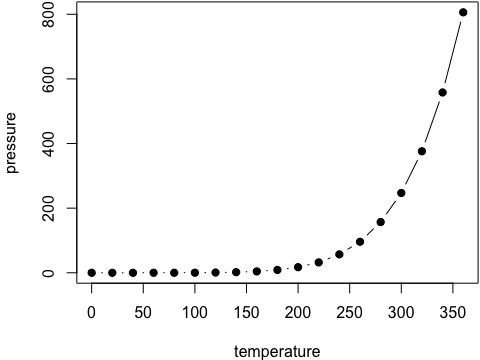
\includegraphics[width=0.8\linewidth]{01-intro_files/figure-latex/nice-fig-01-1} 

}

\caption{Here is a nice figure!}\label{fig:nice-fig-01}
\end{figure}

Reference a figure by its code chunk label with the \texttt{fig:} prefix, e.g., see Figure \ref{fig:nice-fig}. Similarly, you can reference tables generated from \texttt{knitr::kable()}, e.g., see Table \ref{tab:nice-tab}.

\begin{Shaded}
\begin{Highlighting}[]
\NormalTok{knitr}\OperatorTok{::}\KeywordTok{kable}\NormalTok{(}
  \KeywordTok{head}\NormalTok{(iris, }\DecValTok{20}\NormalTok{), }\DataTypeTok{caption =} \StringTok{'Here is a nice table!'}\NormalTok{,}
  \DataTypeTok{booktabs =} \OtherTok{TRUE}
\NormalTok{)}
\end{Highlighting}
\end{Shaded}

\begin{table}

\caption{\label{tab:nice-tab}Here is a nice table!}
\centering
\begin{tabular}[t]{rrrrl}
\toprule
Sepal.Length & Sepal.Width & Petal.Length & Petal.Width & Species\\
\midrule
5.1 & 3.5 & 1.4 & 0.2 & setosa\\
4.9 & 3.0 & 1.4 & 0.2 & setosa\\
4.7 & 3.2 & 1.3 & 0.2 & setosa\\
4.6 & 3.1 & 1.5 & 0.2 & setosa\\
5.0 & 3.6 & 1.4 & 0.2 & setosa\\
\addlinespace
5.4 & 3.9 & 1.7 & 0.4 & setosa\\
4.6 & 3.4 & 1.4 & 0.3 & setosa\\
5.0 & 3.4 & 1.5 & 0.2 & setosa\\
4.4 & 2.9 & 1.4 & 0.2 & setosa\\
4.9 & 3.1 & 1.5 & 0.1 & setosa\\
\addlinespace
5.4 & 3.7 & 1.5 & 0.2 & setosa\\
4.8 & 3.4 & 1.6 & 0.2 & setosa\\
4.8 & 3.0 & 1.4 & 0.1 & setosa\\
4.3 & 3.0 & 1.1 & 0.1 & setosa\\
5.8 & 4.0 & 1.2 & 0.2 & setosa\\
\addlinespace
5.7 & 4.4 & 1.5 & 0.4 & setosa\\
5.4 & 3.9 & 1.3 & 0.4 & setosa\\
5.1 & 3.5 & 1.4 & 0.3 & setosa\\
5.7 & 3.8 & 1.7 & 0.3 & setosa\\
5.1 & 3.8 & 1.5 & 0.3 & setosa\\
\bottomrule
\end{tabular}
\end{table}

You can write citations, too. For example, we are using the \textbf{bookdown} package \citep{R-bookdown} in this sample book, which was built on top of R Markdown and \textbf{knitr} \citep{xie2015}.

\hypertarget{literature}{%
\chapter{Literature}\label{literature}}

Here is a review of existing methods.

\hypertarget{first-graphs}{%
\chapter{First Graphs}\label{first-graphs}}

\hypertarget{les-miserable-dataset}{%
\section{Les Miserable Dataset}\label{les-miserable-dataset}}

\begin{Shaded}
\begin{Highlighting}[]
\CommentTok{# Load igraph}
\KeywordTok{library}\NormalTok{(igraph)}

\CommentTok{# Read data}
\NormalTok{lesmis <-}\StringTok{ }\KeywordTok{read.csv}\NormalTok{(}\StringTok{"https://raw.githubusercontent.com/meefen/sna-ed/master/assets/lesmis/lesmis.csv"}\NormalTok{)}
\CommentTok{# check the head (first 6 rows) of the dataset}
\KeywordTok{head}\NormalTok{(lesmis)}
\end{Highlighting}
\end{Shaded}

\begin{verbatim}
##   Source Target weight
## 1      1      0      1
## 2      2      0      8
## 3      3      0     10
## 4      3      2      6
## 5      4      0      1
## 6      5      0      1
\end{verbatim}

\begin{Shaded}
\begin{Highlighting}[]
\CommentTok{# Create a graph using the graph_from_data_frame function}
\NormalTok{g <-}\StringTok{ }\KeywordTok{graph_from_data_frame}\NormalTok{(lesmis)}

\CommentTok{# Plot the graph}
\KeywordTok{plot}\NormalTok{(g)}
\end{Highlighting}
\end{Shaded}

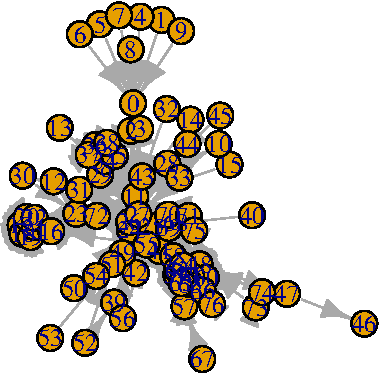
\includegraphics{05-first-charts_files/figure-latex/unnamed-chunk-1-1.pdf}

\begin{Shaded}
\begin{Highlighting}[]
\CommentTok{# make the graph a little prettier}
\KeywordTok{plot}\NormalTok{(g, }\DataTypeTok{edge.arrow.size=}\NormalTok{.}\DecValTok{2}\NormalTok{, }\DataTypeTok{vertex.label=}\OtherTok{NA}\NormalTok{, }\DataTypeTok{vertex.size=}\DecValTok{8}\NormalTok{)}
\end{Highlighting}
\end{Shaded}

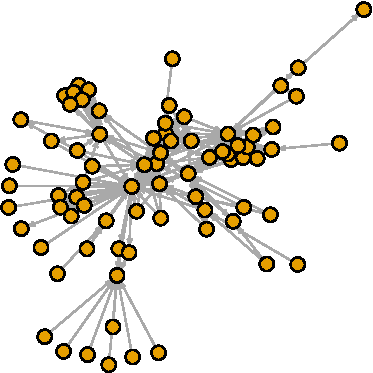
\includegraphics{05-first-charts_files/figure-latex/unnamed-chunk-1-2.pdf}

\hypertarget{stop-light}{%
\section{Stop light}\label{stop-light}}

\begin{Shaded}
\begin{Highlighting}[]
\KeywordTok{library}\NormalTok{(sigmajs)}
\KeywordTok{library}\NormalTok{(tibble)}
\end{Highlighting}
\end{Shaded}

\begin{verbatim}
## 
## Attaching package: 'tibble'
\end{verbatim}

\begin{verbatim}
## The following object is masked from 'package:igraph':
## 
##     as_data_frame
\end{verbatim}

\begin{Shaded}
\begin{Highlighting}[]
\NormalTok{edges <-}\StringTok{ }\KeywordTok{tibble}\NormalTok{(}\DataTypeTok{id =} \KeywordTok{rep}\NormalTok{(}\StringTok{"1"}\NormalTok{, }\DecValTok{3}\NormalTok{),}
                    \DataTypeTok{source =} \KeywordTok{rep}\NormalTok{(}\StringTok{"1"}\NormalTok{, }\DecValTok{3}\NormalTok{),}
                    \DataTypeTok{target =} \KeywordTok{as.character}\NormalTok{(}\KeywordTok{c}\NormalTok{(}\DecValTok{2}\OperatorTok{:}\DecValTok{4}\NormalTok{))}
\NormalTok{                    )}
\NormalTok{nodes <-}\StringTok{ }\KeywordTok{tibble}\NormalTok{(}\DataTypeTok{id =} \KeywordTok{as.character}\NormalTok{(}\DecValTok{1}\OperatorTok{:}\DecValTok{4}\NormalTok{),}
                    \DataTypeTok{label =} \KeywordTok{c}\NormalTok{(}\StringTok{"light"}\NormalTok{, }\StringTok{"red"}\NormalTok{, }\StringTok{"yellow"}\NormalTok{, }\StringTok{"green"}\NormalTok{),}
                    \DataTypeTok{time =} \KeywordTok{c}\NormalTok{(}\DecValTok{100}\NormalTok{, }\DecValTok{30}\NormalTok{, }\DecValTok{10}\NormalTok{, }\DecValTok{20}\NormalTok{)}
\NormalTok{)}
\KeywordTok{sigmajs}\NormalTok{() }\OperatorTok
\StringTok{  }\KeywordTok{sg_nodes}\NormalTok{(nodes, id, label, time) }\OperatorTok
\StringTok{  }\KeywordTok{sg_edges}\NormalTok{(edges, id, source, target) }
\end{Highlighting}
\end{Shaded}


\includegraphics{05-first-charts_files/figure-latex/unnamed-chunk-2-1.pdf}

\hypertarget{les-miserabe}{%
\section{Les Miserabe}\label{les-miserabe}}

\hypertarget{sigma}{%
\chapter{Sigma JS}\label{sigma}}

\begin{Shaded}
\begin{Highlighting}[]
\CommentTok{#example for ?sigmajs::sigmajs}
\KeywordTok{library}\NormalTok{(sigmajs)}
\NormalTok{nodes <-}\StringTok{ }\KeywordTok{sg_make_nodes}\NormalTok{()}
\NormalTok{edges <-}\StringTok{ }\KeywordTok{sg_make_edges}\NormalTok{(nodes)}

\KeywordTok{sigmajs}\NormalTok{() }\OperatorTok
\StringTok{  }\KeywordTok{sg_nodes}\NormalTok{(nodes, id, label, size, color) }\OperatorTok
\StringTok{  }\KeywordTok{sg_edges}\NormalTok{(edges, id, source, target) }
\end{Highlighting}
\end{Shaded}


\includegraphics{06-sigma_files/figure-latex/unnamed-chunk-2-1.pdf}

\hypertarget{stop-light-1}{%
\section{Stop light}\label{stop-light-1}}

\begin{Shaded}
\begin{Highlighting}[]
\KeywordTok{library}\NormalTok{(sigmajs)}
\KeywordTok{library}\NormalTok{(tibble)}
\NormalTok{edges <-}\StringTok{ }\KeywordTok{tibble}\NormalTok{(}\DataTypeTok{id =} \KeywordTok{rep}\NormalTok{(}\StringTok{"1"}\NormalTok{, }\DecValTok{3}\NormalTok{),}
                    \DataTypeTok{source =} \KeywordTok{rep}\NormalTok{(}\StringTok{"1"}\NormalTok{, }\DecValTok{3}\NormalTok{),}
                    \DataTypeTok{target =} \KeywordTok{as.character}\NormalTok{(}\KeywordTok{c}\NormalTok{(}\DecValTok{2}\OperatorTok{:}\DecValTok{4}\NormalTok{))}
\NormalTok{                    )}
\NormalTok{nodes <-}\StringTok{ }\KeywordTok{tibble}\NormalTok{(}\DataTypeTok{id =} \KeywordTok{as.character}\NormalTok{(}\DecValTok{1}\OperatorTok{:}\DecValTok{4}\NormalTok{),}
                    \DataTypeTok{label =} \KeywordTok{c}\NormalTok{(}\StringTok{"light"}\NormalTok{, }\StringTok{"red"}\NormalTok{, }\StringTok{"yellow"}\NormalTok{, }\StringTok{"green"}\NormalTok{),}
                    \DataTypeTok{time =} \KeywordTok{c}\NormalTok{(}\DecValTok{100}\NormalTok{, }\DecValTok{30}\NormalTok{, }\DecValTok{10}\NormalTok{, }\DecValTok{20}\NormalTok{)}
\NormalTok{)}
\KeywordTok{sigmajs}\NormalTok{() }\OperatorTok
\StringTok{  }\KeywordTok{sg_nodes}\NormalTok{(nodes, id, label, time) }\OperatorTok
\StringTok{  }\KeywordTok{sg_edges}\NormalTok{(edges, id, source, target) }
\end{Highlighting}
\end{Shaded}


\includegraphics{06-sigma_files/figure-latex/unnamed-chunk-3-1.pdf}

\hypertarget{glossary}{%
\chapter{Glossary}\label{glossary}}

\textbf{Attributes} are a characteristic of the node or edge that is often designated by color, size, or shape of the object. For example, a dashed line for an edge or a blue circle for a node.

\textbf{Nodes} are also actors or vertices. They are things like people, places, ideas that have some connection. In mathmatical formulas, they often take the variable \(N\).

\textbf{Degree} the number of nodes adjacent to the node under evaluation or the number of lines incident to it.

\textbf{Diameter} is the maximum number of edges.

\textbf{Edges} are ties, relations or connections between nodes. Edges are often designated as \(E\).

\textbf{Indegree} is the number of received ties.

\textbf{Networks}

\textbf{Network objects} is a class of objects in R designed specifically for network analysis. They store an adjacency matrix or an edgelist as well as metadata.

\textbf{Outdegree} the number of sent ties.

\textbf{Directed} networks

\bibliography{book.bib,packages.bib}

\end{document}
